\documentclass[]{article}

\usepackage{graphicx}

%opening
\title{3D motion planning project}
\author{Juan Irving Vasquez-Gomez}

\begin{document}

\maketitle

%\begin{abstract}

%\end{abstract}

\section{PRM planner}

The probabilistic road map (PRM) [1] is a sampling based motion planning algorithm. It generates random points inside the workspace verifying that they are collision free. Then it connects the points by constructing a graph among those points. 

In this project, I have implemented a PRM. The random points are generated inside the city and each point is verified to be collision free. To connect the points I check that the line between those points does not intersect any of  the building polygons. Fig. shows an example of the generated graph.

\begin{figure}
\centering
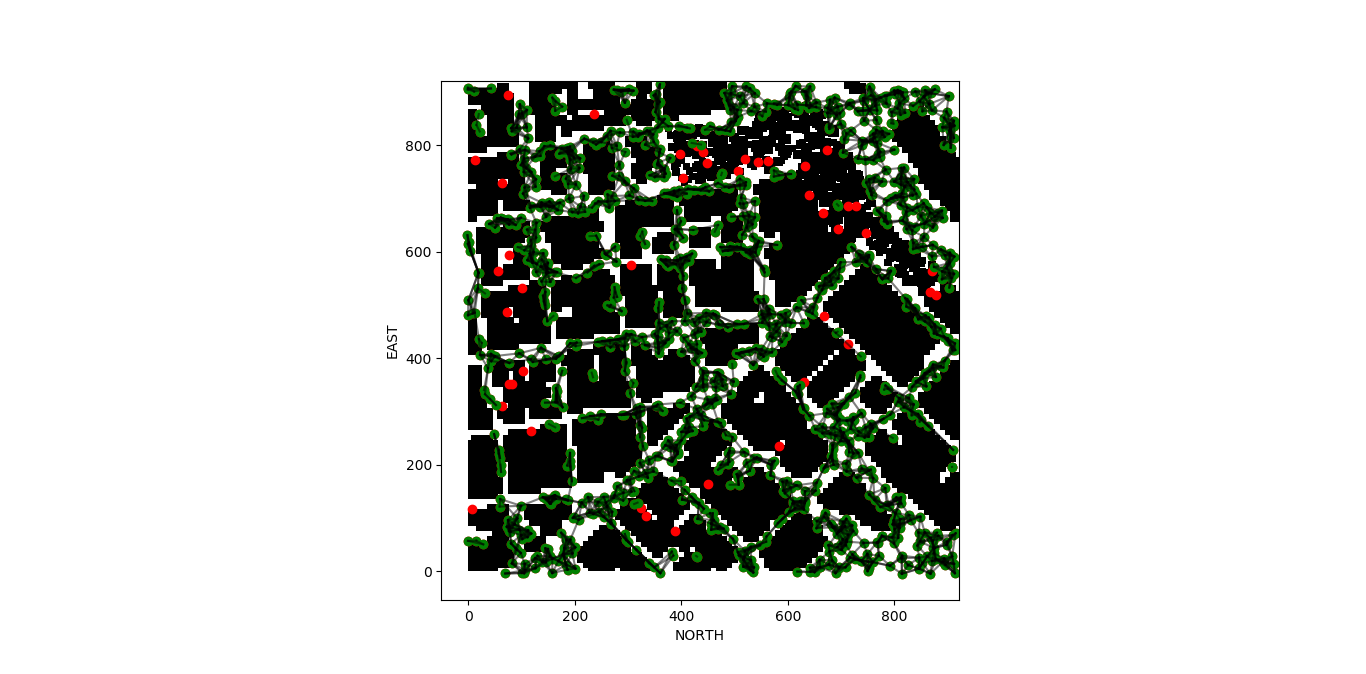
\includegraphics[width=\linewidth, trim={11cm 1cm 11cm 2cm}, clip]{graph}
\caption{Example of the graph. Green dots are connected vertices, red dots are unconnected vertices. 3000 random samples were drawn, keeping only 1237 feasible samples. Each vertex was tried to be connected with seven nearest neighbors. }
\label{fig:graph}
\end{figure}


To find a path between the current position  and a goal position. First, the nearest vertices in the graph are found, then a feasible path is found using A*. Fig. shows and example of a computed path.

\begin{figure}
\centering
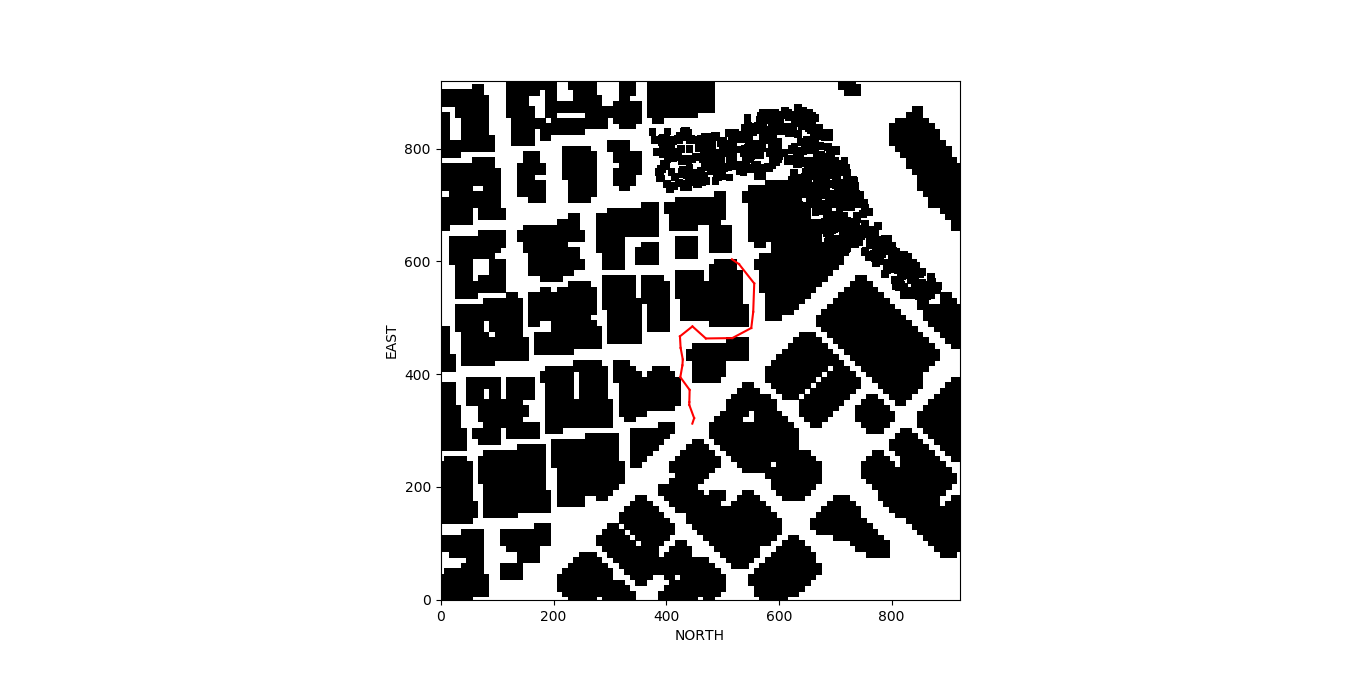
\includegraphics[width=\linewidth, trim={11cm 1cm 11cm 2cm}, clip]{path}
\caption{Example of a computed path.}
\label{fig:path}
\end{figure}

\section{Specifications}


\subsection{Explain the starter code}

motion\_planning.py is the main script. It is a child class from Drone class. It is in charge of communicating with the drone and it reacts depending on the events coming from the drone. 

The class follows the event programming paradigm. When the program starts, in \texttt{state\_callback()} function the drone goes from MANUAL state to ARMING, PLANNING, TAKE\_OFF, WAYPOINT, LANDING and DISARMING.

For planning the path the \texttt{plan\_path()} function is used. Inside this function an arbitrary goal is defined. Then, A* is used to plan the path to such goal. A* uses an euclidean distance and all the actions have the same cost and they move the drone only in a 2D plane.

\subsection{Local position}

\begin{verbatim}
	# TODO: set home position to (lon0, lat0, 0)
	self.set_home_position(lon0, lat0, 0)
	
	# TODO: retrieve current global position
	geo_current = self.global_position
	print("my currrent global position:", geo_current)
	
	# TODO: convert to current local position using global_to_local()
	ned_current = global_to_local(geo_current, self.global_home)
\end{verbatim}

\subsection{Setting the start point}

\begin{verbatim}
	# TODO: convert to current local position using global_to_local()
	ned_current = global_to_local(geo_current, self.global_home)
	
	#find the closest node
	closest_start = prm.closest_point(self.prm_g, (ned_current[0], ned_current[1], TARGET_ALTITUDE))
\end{verbatim}

\subsection{Geodetic goal}

I generate the geodetic goal randomly

\begin{verbatim}
# assuming that home is the center
geo_min = local_to_global([north_offset, east_offset, 0], self.global_home)
geo_max = local_to_global([-north_offset, -east_offset, 0], self.global_home)
random = np.random.rand(3)

geo_goal = geo_min + (np.multiply(geo_max-geo_min, random))

print('Geodetic goal: ', geo_goal)
ned_goal = global_to_local(geo_goal, self.global_home)

\end{verbatim}

\section{Issues}

I found that when many waypoints are send to be displayed the program broke dawn. In some cases the drone makes rare movements. 

\section{Conclusions}

A possible way to find the path between two points is to use the probabilistic road map (PRM). Once that the road map has been created, it is very fast to get a path. However, the graph construction is a long time consuming process. The current planner can be improved by getting a coarse plan using the PRM and then refine it using grid based A* between each configuration of the coarse plan.

\section{References}

1. 

\end{document}
